\documentclass[11pt,a4paper]{report}
\usepackage[textwidth=37em,vmargin=30mm]{geometry}
\usepackage{calc,xunicode,amsmath,amssymb,paralist,enumitem,tabu,booktabs,datetime2,xeCJK,xeCJKfntef,listings}
\usepackage{tocloft,fancyhdr,tcolorbox,xcolor,graphicx,eso-pic,xltxtra,xelatexemoji}

\newcommand{\envyear}[0]{2025}
\newcommand{\envdatestr}[0]{2025-04-05}
\newcommand{\envfinaldir}[0]{webdb/2025/20250405/final}

\usepackage[hidelinks]{hyperref}
\hypersetup{
    colorlinks=false,
    pdfpagemode=FullScreen,
    pdftitle={Web Digest - \envdatestr}
}

\setlength{\cftbeforechapskip}{10pt}
\renewcommand{\cftchapfont}{\rmfamily\bfseries\large\raggedright}
\setlength{\cftbeforesecskip}{2pt}
\renewcommand{\cftsecfont}{\sffamily\small\raggedright}

\setdefaultleftmargin{2em}{2em}{1em}{1em}{1em}{1em}

\usepackage{xeCJK,xeCJKfntef}
\xeCJKsetup{PunctStyle=plain,RubberPunctSkip=false,CJKglue=\strut\hskip 0pt plus 0.1em minus 0.05em,CJKecglue=\strut\hskip 0.22em plus 0.2em}
\XeTeXlinebreaklocale "zh"
\XeTeXlinebreakskip = 0pt


\setmainfont{Brygada 1918}
\setromanfont{Brygada 1918}
\setsansfont{IBM Plex Sans}
\setmonofont{JetBrains Mono NL}
\setCJKmainfont{Noto Serif CJK SC}
\setCJKromanfont{Noto Serif CJK SC}
\setCJKsansfont{Noto Sans CJK SC}
\setCJKmonofont{Noto Sans CJK SC}

\setlength{\parindent}{0pt}
\setlength{\parskip}{8pt}
\linespread{1.15}

\lstset{
	basicstyle=\ttfamily\footnotesize,
	numbersep=5pt,
	backgroundcolor=\color{black!5},
	showspaces=false,
	showstringspaces=false,
	showtabs=false,
	tabsize=2,
	captionpos=b,
	breaklines=true,
	breakatwhitespace=true,
	breakautoindent=true,
	linewidth=\textwidth
}






\newcommand{\coverpic}[2]{
    % argv: itemurl, authorname
    Cover photo by #2~~(\href{#1}{#1})
}
\newcommand{\makeheader}[0]{
    \begin{titlepage}
        % \newgeometry{hmargin=15mm,tmargin=21mm,bmargin=12mm}
        \begin{center}
            
            \rmfamily\scshape
            \fontspec{BaskervilleF}
            \fontspec{Old Standard}
            \fontsize{59pt}{70pt}\selectfont
            WEB\hfill DIGEST
            
            \vfill
            % \vskip 30pt
            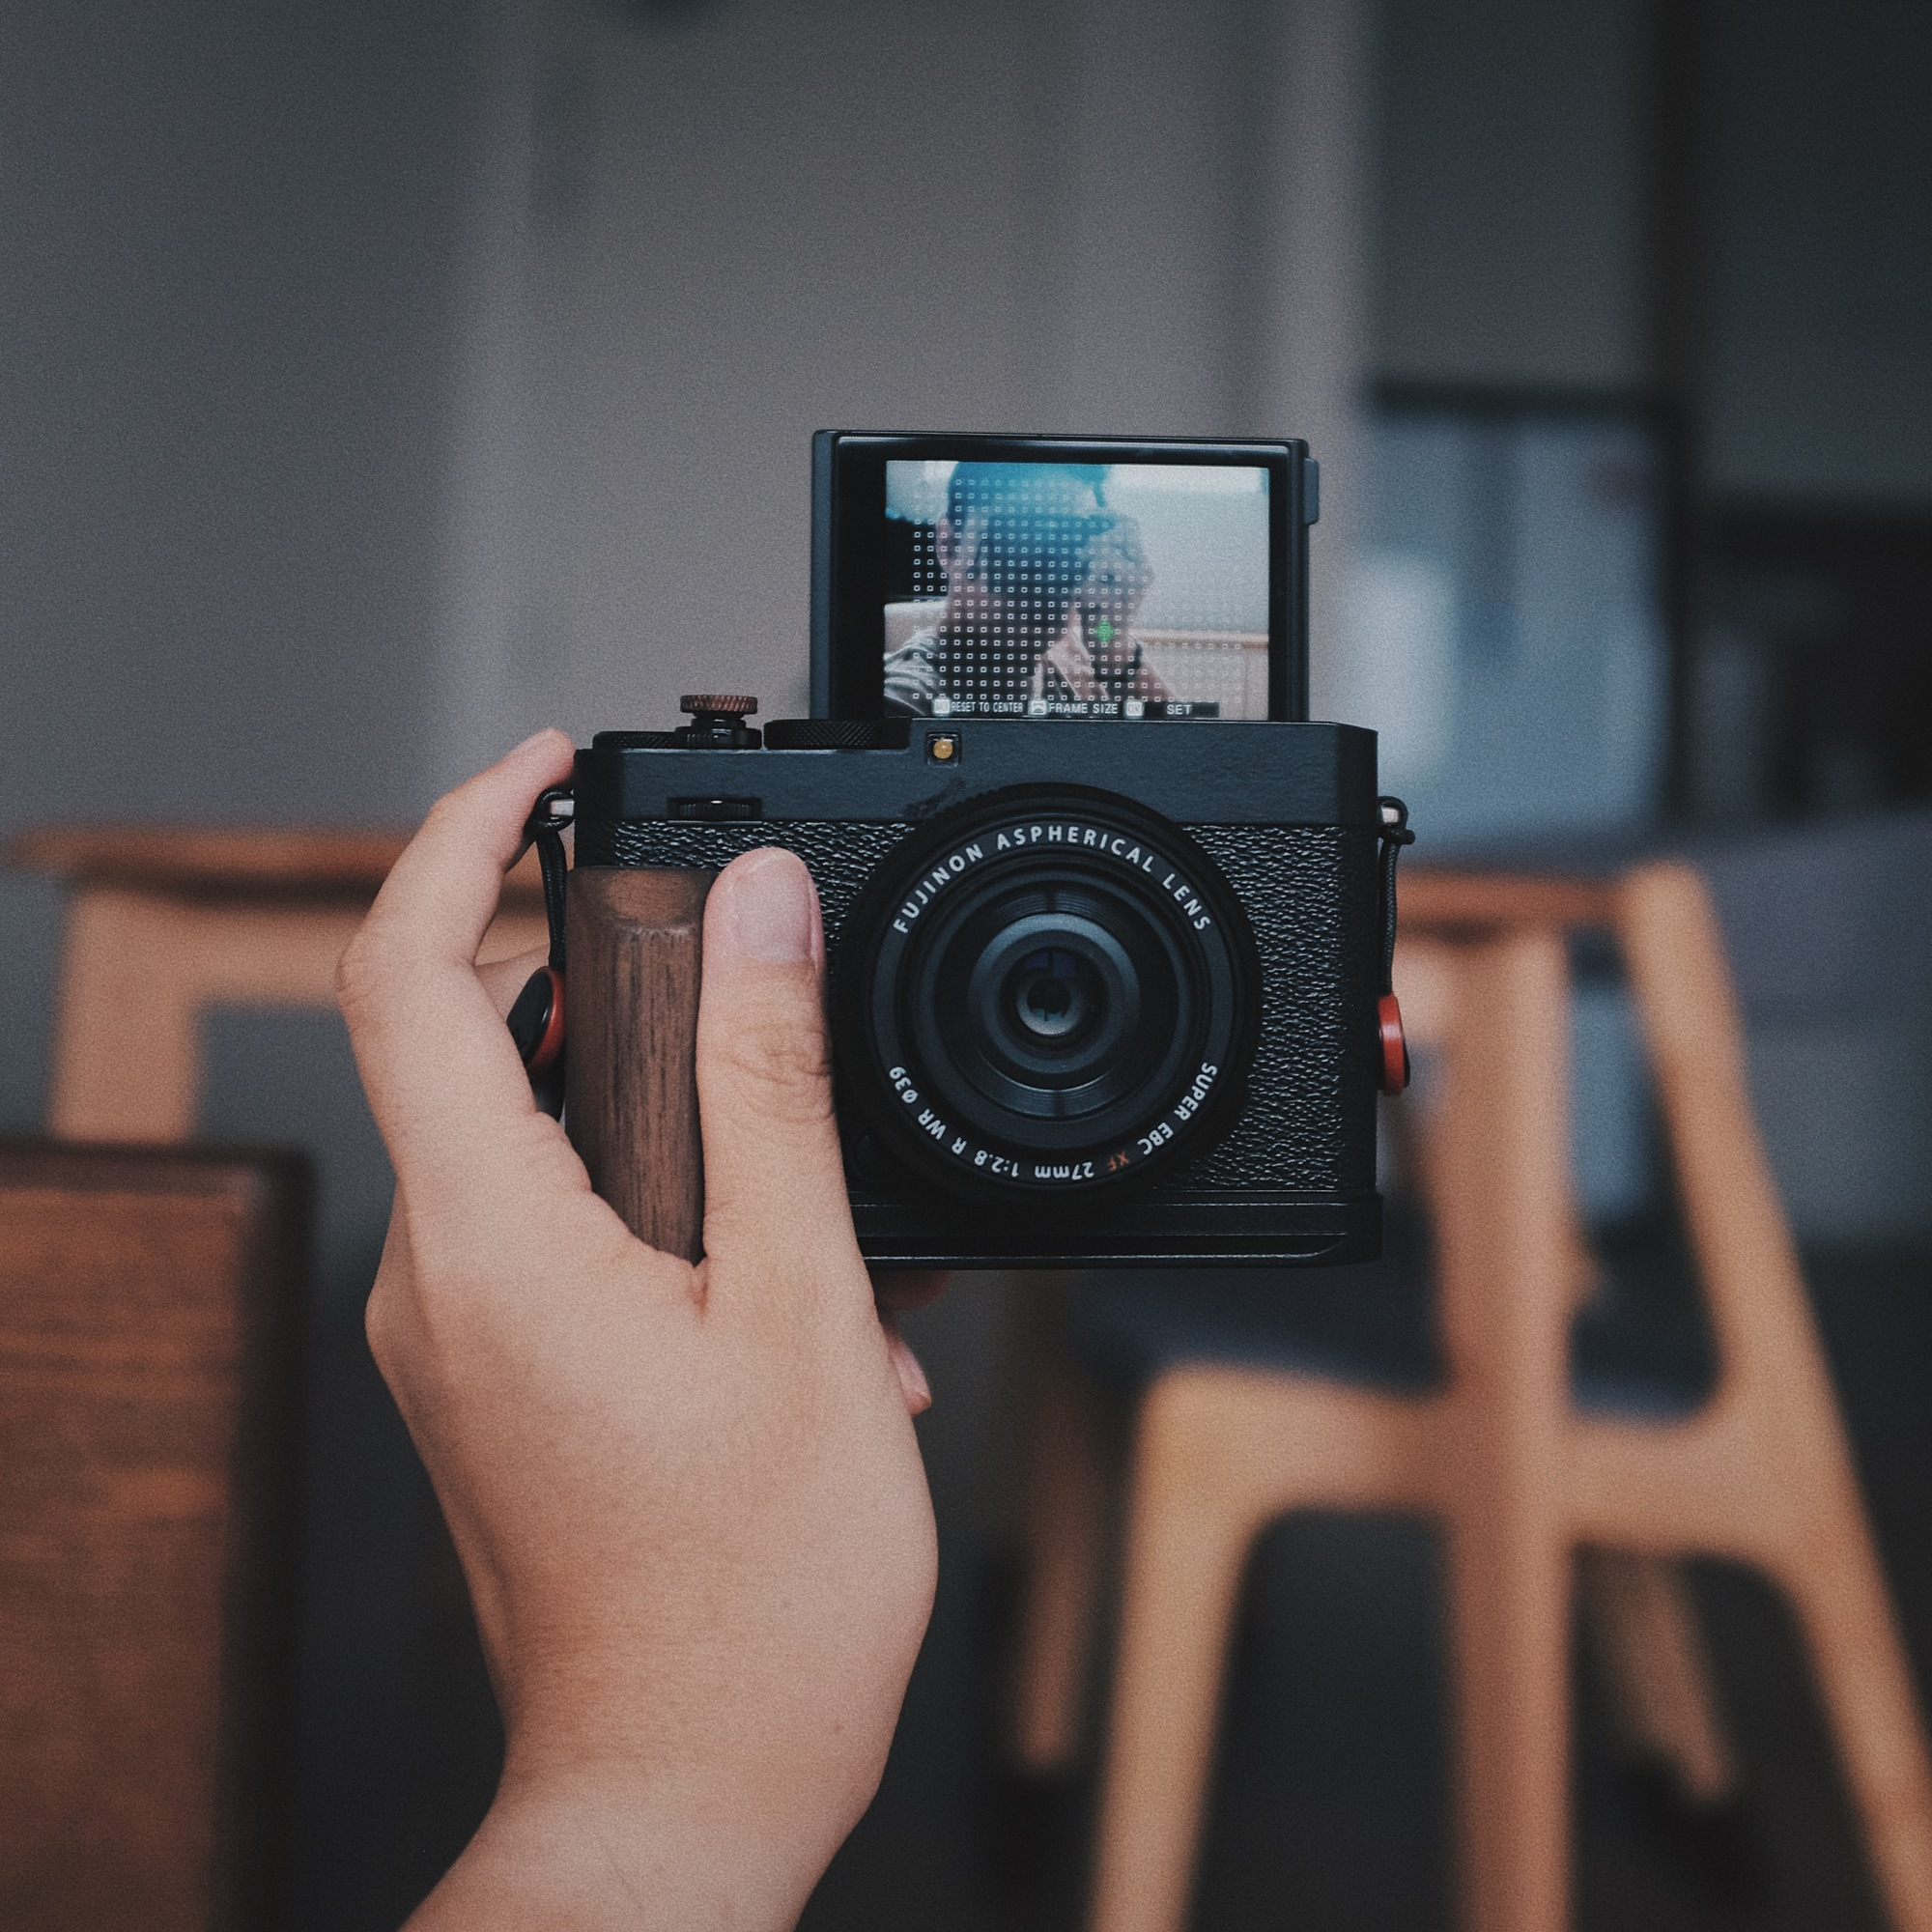
\includegraphics[width=\linewidth]{\envfinaldir/coverpic-prod.jpg}\par
            % \vskip 30pt
            \vfill

            \normalsize\rmfamily\scshape
            \copyright{} The Web Digest Project \hfill\large \envdatestr
        \end{center}
    \end{titlepage}
    % \restoregeometry
}
\newcommand{\simplehref}[1]{%
    \textcolor{blue!80!green}{\href{#1}{#1}}%
}
\renewcommand{\contentsname}{\center\Huge\sffamily\bfseries Contents\par\vskip 20pt}
\newcounter{ipartcounter}
\setcounter{ipartcounter}{0}
\newcommand{\ipart}[1]{
    % \vskip 20pt
    \clearpage
    \stepcounter{ipartcounter}
    \phantomsection
    \addcontentsline{toc}{chapter}{#1}
    % \begin{center}
    %     \Huge
    %     \sffamily\bfseries
    %     #1
    % \end{center}
    % \vskip 20pt plus 7pt
}
\newcounter{ichaptercounter}
\setcounter{ichaptercounter}{0}
\newcommand{\ichapter}[1]{
    % \vskip 20pt
    \clearpage
    \stepcounter{ichaptercounter}
    \phantomsection
    \addcontentsline{toc}{section}{\numberline{\arabic{ichaptercounter}}#1}
    \begin{center}
        \Huge
        \sffamily\bfseries
        #1
    \end{center}
    \vskip 20pt plus 7pt
}
\newcommand{\entrytitlefont}[1]{\subsection*{\raggedright\Large\sffamily\bfseries#1}}
\newcommand{\entryitemGeneric}[2]{
    % argv: title, url
    \parbox{\linewidth}{
        \entrytitlefont{#1}\par\vskip 5pt
        \footnotesize\ttfamily\mdseries
        \simplehref{#2}
    }\vskip 11pt plus 11pt minus 1pt
}
\newcommand{\entryitemGithub}[3]{
    % argv: title, url, desc
    \parbox{\linewidth}{
        \entrytitlefont{#1}\par\vskip 5pt
        \footnotesize\ttfamily\mdseries
        \simplehref{#2}\par\vskip 5pt
        \small\rmfamily\mdseries#3
    }\vskip 11pt plus 11pt minus 1pt
}
\newcommand{\entryitemAp}[3]{
    % argv: title, url, desc
    \parbox{\linewidth}{
        \entrytitlefont{#1}\par\vskip 5pt
        \footnotesize\ttfamily\mdseries
        \simplehref{#2}\par\vskip 5pt
        \small\rmfamily\mdseries#3
    }\vskip 11pt plus 11pt minus 1pt
}
\newcommand{\entryitemHackernews}[3]{
    % argv: title, hnurl, rawurl
    % \parbox{\linewidth}{
    %     \entrytitlefont{#1}\par\vskip 5pt
    %     \footnotesize\ttfamily\mdseries
    %     \simplehref{#3}\par
    %     \textcolor{black!50}{\href{#2}{#2}}
    % }\vskip 11pt plus 11pt minus 1pt
    \begin{minipage}{\linewidth}
            \entrytitlefont{#1}\par\vskip 5pt
            \footnotesize\ttfamily\mdseries
            \simplehref{#3}\par
            \textcolor{black!50}{\href{#2}{#2}}
    \end{minipage}\par\vskip 11pt plus 11pt minus 1pt
}







\begin{document}

\makeheader

\tableofcontents\clearpage




\ipart{Developers}
\ichapter{Hacker News}
\entryitemTwoLinks{Dow plunges 2,200 points, Nasdaq enters bear market}{https://news.ycombinator.com/item?id=43587479}{https://finance.yahoo.com/news/live/stock-market-today-dow-plunges-2200-points-nasdaq-enters-bear-market-as-trump-tariffs-spark-worst-meltdown-since-2020-200042876.html}

\entryitemTwoLinks{The blissful Zen of a good side project}{https://news.ycombinator.com/item?id=43587380}{https://joshcollinsworth.com/blog/the-blissful-zen-of-a-good-side-project}

\entryitemTwoLinks{Google announces Sec-Gemini v1 a new experimental cybersecurity model}{https://news.ycombinator.com/item?id=43586786}{https://security.googleblog.com/2025/04/google-launches-sec-gemini-v1-new.html}

\entryitemTwoLinks{An interactive-speed Linux computer made of only 3 8-pin chips}{https://news.ycombinator.com/item?id=43586654}{https://dmitry.gr/?r=05.Projects\&proj=36.\%208pinLinux}

\entryitemTwoLinks{The End of Sierra as We Knew It, Part 1: The Acquisition}{https://news.ycombinator.com/item?id=43586157}{https://www.filfre.net/2025/04/the-end-of-sierra-as-we-knew-it-part-1-the-acquisition/}

\entryitemTwoLinks{Gumroad's license wouldn't meet the widely regarded definition of open source}{https://news.ycombinator.com/item?id=43586107}{https://danb.me/blog/gumroad-is-not-open-source/}

\entryitemTwoLinks{Understanding Machine Learning: From Theory to Algorithms}{https://news.ycombinator.com/item?id=43586073}{https://www.cs.huji.ac.il/~shais/UnderstandingMachineLearning/copy.html}

\entryitemTwoLinks{The Curse of Ayn Rand's Heir}{https://news.ycombinator.com/item?id=43584663}{https://www.theatlantic.com/ideas/archive/2025/03/ayn-rand-peikoff-inheritance-battle/682219/}

\entryitemTwoLinks{Kerosene did not save the sperm whale (2024)}{https://news.ycombinator.com/item?id=43584303}{https://edconway.substack.com/p/no-kerosene-did-not-save-the-sperm}

\entryitemTwoLinks{Wealthy Americans have death rates on par with poor Europeans}{https://news.ycombinator.com/item?id=43584156}{https://arstechnica.com/health/2025/04/wealthy-americans-have-death-rates-on-par-with-poor-europeans/}

\entryitemTwoLinks{Dow Slides Another 1k Points. Nasdaq on Pace to Enter Bear Market}{https://news.ycombinator.com/item?id=43582292}{https://www.barrons.com/livecoverage/stock-market-today-040425}

\entryitemTwoLinks{Why does Britain feel so poor?}{https://news.ycombinator.com/item?id=43581672}{https://martinrobbins.substack.com/p/von-6-why-does-britain-feel-so-poor}

\entryitemTwoLinks{Nvidia adds native Python support to CUDA}{https://news.ycombinator.com/item?id=43581584}{https://thenewstack.io/nvidia-finally-adds-native-python-support-to-cuda/}

\entryitemTwoLinks{Trump's Trade War Escalates as China Retaliates with 34\% Tariffs}{https://news.ycombinator.com/item?id=43580906}{https://www.nytimes.com/2025/04/04/business/china-trump-tariffs-retaliation.html}

\entryitemTwoLinks{Bored of It}{https://news.ycombinator.com/item?id=43580449}{https://paulrobertlloyd.com/2025/087/a1/bored/}

\entryitemTwoLinks{Gumroad's source is available}{https://news.ycombinator.com/item?id=43580103}{https://github.com/antiwork/gumroad}

\entryitemTwoLinks{Doge staffer's YouTube nickname accidentally revealed his teen hacking activity}{https://news.ycombinator.com/item?id=43579925}{https://arstechnica.com/tech-policy/2025/04/i-no-longer-hack-paypals-doge-staffers-hacker-past-raises-red-flags/}

\entryitemTwoLinks{Growing trade deficit is selling the nation out from under us (2003) [pdf]}{https://news.ycombinator.com/item?id=43579908}{https://faculty.washington.edu/ss1110/IF/Buffett\%20Fortune\%202003\%20(6).pdf}

\entryitemTwoLinks{Head of NSA and Cybercommand Is Ousted}{https://news.ycombinator.com/item?id=43578475}{https://www.nytimes.com/2025/04/03/us/politics/nsa-cyber-command-chief-fired.html}

\entryitemTwoLinks{DeepSeek: Inference-Time Scaling for Generalist Reward Modeling}{https://news.ycombinator.com/item?id=43578430}{https://arxiv.org/abs/2504.02495}\ichapter{Phoronix}
\entryitemGeneric{\hskip 0pt{}Wine 10.5 Brings Vulkan H.264 Video Decoding, Mono 10.0 \& Bluetooth Pairing}{https://www.phoronix.com/news/Wine-10.5-Released}

\entryitemGeneric{\hskip 0pt{}Vulkan 1.4.312 Brings Two New Extensions From NVIDIA \& Qualcomm}{https://www.phoronix.com/news/Vulkan-1.4.312-Released}

\entryitemGeneric{\hskip 0pt{}Linux 6.15 USB/Thunderbolt Changes Include The New PS883X Driver}{https://www.phoronix.com/news/Linux-6.15-USB}

\entryitemGeneric{\hskip 0pt{}Rust Is Looking For Your Feedback To Help Guide Its Future}{https://www.phoronix.com/news/Rust-Vision-Survey-2025}

\entryitemGeneric{\hskip 0pt{}AMD RDNA 3.5 Graphics On 2025 Drivers: Windows 11 vs. Ubuntu 25.04 iGPU Performance}{https://www.phoronix.com/review/amd-rdna35-ubuntu-2504}

\entryitemGeneric{\hskip 0pt{}ZLUDA Continues Working On PyTorch Support, Eyes 32-bit PhysX Support}{https://www.phoronix.com/news/ZLUDA-Q1-2025}

\entryitemGeneric{\hskip 0pt{}NVIDIA Engineer Fixes Early Linux 6.15 Performance Regression Affecting AMD GPU Drivers}{https://www.phoronix.com/news/Linux-6.15-Early-AMD-Regression}

\entryitemGeneric{\hskip 0pt{}Linux Bring-Up For The Apple M4 Looks Like It Will Be "Rather Painful"}{https://www.phoronix.com/news/Apple-M4-Linux-Rather-Painful}

\entryitemGeneric{\hskip 0pt{}MSEAL Protection Of System Mappings Merged For Linux 6.15}{https://www.phoronix.com/news/Linux-6.15-MSEAL-System-Mapping}\ichapter{Dribbble}
\entryitemGeneric{\hskip 0pt{}Educational Website on Space Pollution}{https://dribbble.com/shots/25860515-Educational-Website-on-Space-Pollution}

\entryitemGeneric{\hskip 0pt{}CRYSTAL PRT\_2 // Mobile Version}{https://dribbble.com/shots/25860264-CRYSTAL-PRT-2-Mobile-Version}

\entryitemGeneric{\hskip 0pt{}Ship Logo Design - Boat, Shield, Star, Waves}{https://dribbble.com/shots/25854151-Ship-Logo-Design-Boat-Shield-Star-Waves}

\entryitemGeneric{\hskip 0pt{}HR website}{https://dribbble.com/shots/25854264-HR-website}

\entryitemGeneric{\hskip 0pt{}Interactive Speed Slider}{https://dribbble.com/shots/25851176-Interactive-Speed-Slider}

\entryitemGeneric{\hskip 0pt{}Abstract}{https://dribbble.com/shots/25853030-Abstract}

\entryitemGeneric{\hskip 0pt{}Croc logo}{https://dribbble.com/shots/25852607-Croc-logo}

\entryitemGeneric{\hskip 0pt{}Logo Design Selection Q1 2025}{https://dribbble.com/shots/25852275-Logo-Design-Selection-Q1-2025}

\entryitemGeneric{\hskip 0pt{}Cloud Lightning}{https://dribbble.com/shots/25852815-Cloud-Lightning}

\entryitemGeneric{\hskip 0pt{}Jot Landing Page, Website Design, business web site}{https://dribbble.com/shots/25843658-Jot-Landing-Page-Website-Design-business-web-site}

\entryitemGeneric{\hskip 0pt{}ef monogram}{https://dribbble.com/shots/25847206-ef-monogram}

\entryitemGeneric{\hskip 0pt{}Helpfull - Logo Redesign}{https://dribbble.com/shots/25847828-Helpfull-Logo-Redesign}

\entryitemGeneric{\hskip 0pt{}Outrigger Marketing Logo}{https://dribbble.com/shots/25848681-Outrigger-Marketing-Logo}

\entryitemGeneric{\hskip 0pt{}Wayflow Logo Design - Letter W, Waves, Flow}{https://dribbble.com/shots/25847473-Wayflow-Logo-Design-Letter-W-Waves-Flow}

\entryitemGeneric{\hskip 0pt{}Letter G set}{https://dribbble.com/shots/25845864-Letter-G-set}

\entryitemGeneric{\hskip 0pt{}Vínföng Final Wordmark}{https://dribbble.com/shots/25848505-V-nf-ng-Final-Wordmark}

\entryitemGeneric{\hskip 0pt{}Prana Symbol}{https://dribbble.com/shots/25847656-Prana-Symbol}

\entryitemGeneric{\hskip 0pt{}Let down your hair}{https://dribbble.com/shots/25844844-Let-down-your-hair}

\entryitemGeneric{\hskip 0pt{}Chat GPT 4 Branding Concept}{https://dribbble.com/shots/25844194-Chat-GPT-4-Branding-Concept}

\entryitemGeneric{\hskip 0pt{}Sustainable contribution selector: percentage picker}{https://dribbble.com/shots/25843734-Sustainable-contribution-selector-percentage-picker}

\entryitemGeneric{\hskip 0pt{}FG}{https://dribbble.com/shots/25842733-FG}

\entryitemGeneric{\hskip 0pt{}Kovre Winery Logo Exploration}{https://dribbble.com/shots/25844706-Kovre-Winery-Logo-Exploration}

\entryitemGeneric{\hskip 0pt{}Cloud Paper}{https://dribbble.com/shots/25844908-Cloud-Paper}

\entryitemGeneric{\hskip 0pt{}Crypto Portfolio Dashboard}{https://dribbble.com/shots/25841268-Crypto-Portfolio-Dashboard}


\ipart{Developers~~~~(zh-Hans)}
\ichapter{Solidot}
\entryitemGeneric{\hskip 0pt{}朝鲜黑客如何窃取数以十亿美元的加密货币}{https://www.solidot.org/story?sid=80967}

\entryitemGeneric{\hskip 0pt{}美国 34 家比特币矿场的耗电量超过洛杉矶}{https://www.solidot.org/story?sid=80966}

\entryitemGeneric{\hskip 0pt{}小行星 2024 YR4 撞击月球概率上调至 3.8\%}{https://www.solidot.org/story?sid=80965}

\entryitemGeneric{\hskip 0pt{}盖茨以 PDF 形式发布了 Altair BASIC 源代码}{https://www.solidot.org/story?sid=80964}

\entryitemGeneric{\hskip 0pt{}美国富人的寿命低于欧洲富人}{https://www.solidot.org/story?sid=80963}

\entryitemGeneric{\hskip 0pt{}部分音乐享受能力或来自遗传}{https://www.solidot.org/story?sid=80962}

\entryitemGeneric{\hskip 0pt{}微软 CTO 预测五年内 95\% 的代码由 AI 生成}{https://www.solidot.org/story?sid=80961}

\entryitemGeneric{\hskip 0pt{}雄性果蝇饮酒能增加对雌性的吸引力}{https://www.solidot.org/story?sid=80960}

\entryitemGeneric{\hskip 0pt{}PorteuX 2.0 释出}{https://www.solidot.org/story?sid=80959}

\entryitemGeneric{\hskip 0pt{}维基基金会称 AI 爬虫导致带宽消耗增加五成}{https://www.solidot.org/story?sid=80958}

\entryitemGeneric{\hskip 0pt{}任天堂将第一方游戏售价提高到 70/80 美元}{https://www.solidot.org/story?sid=80957}

\entryitemGeneric{\hskip 0pt{}丢弃的锂离子电池引发火灾}{https://www.solidot.org/story?sid=80956}

\entryitemGeneric{\hskip 0pt{}贝莱德 CEO 称比特币可能取代美元成为全世界的储备货币}{https://www.solidot.org/story?sid=80955}

\entryitemGeneric{\hskip 0pt{}Rockbox 4.0 释出}{https://www.solidot.org/story?sid=80954}

\entryitemGeneric{\hskip 0pt{}Switch 2 将于 6 月 5 日上市,起售价 450 美元}{https://www.solidot.org/story?sid=80953}

\entryitemGeneric{\hskip 0pt{}Steam 平台的 Linux 份额达到 2.33\%}{https://www.solidot.org/story?sid=80952}

\entryitemGeneric{\hskip 0pt{}到本世纪末如果全球气温上升 3°C 全世界四成经济可能会被抹掉}{https://www.solidot.org/story?sid=80951}

\entryitemGeneric{\hskip 0pt{}年轻男性泡冷水澡或有助于身体健康}{https://www.solidot.org/story?sid=80950}

\entryitemGeneric{\hskip 0pt{}每周三天间歇性禁食减肥效果显著}{https://www.solidot.org/story?sid=80949}

\entryitemGeneric{\hskip 0pt{}OpenAI 被指控未经授权使用 O'Reilly 书籍训练 GPT-4o}{https://www.solidot.org/story?sid=80948}\ichapter{V2EX}
\entryitemGeneric{\hskip 0pt{}[Windows] Windows 热更新体验开始支持 Windows 11 24H2 企业版}{https://www.v2ex.com/t/1123352}

\entryitemGeneric{\hskip 0pt{}[分享创造] 我是如何管理独立开发项目的?一个拒绝拖延的极简工作流}{https://www.v2ex.com/t/1123351}

\entryitemGeneric{\hskip 0pt{}[macOS] 提醒大家一下 15.4}{https://www.v2ex.com/t/1123350}

\entryitemGeneric{\hskip 0pt{}[macOS] 用 mac 的妙控板如何左右切换浏览器的 tab?}{https://www.v2ex.com/t/1123349}

\entryitemGeneric{\hskip 0pt{}[软件] 只考虑 Android 平台国产 app 的补全体验,哪个密码管理器最好?}{https://www.v2ex.com/t/1123348}

\entryitemGeneric{\hskip 0pt{}[分享发现] 比尔盖茨的 Blog 的 UI 好好看啊}{https://www.v2ex.com/t/1123346}

\entryitemGeneric{\hskip 0pt{}[成都] 买五城区的老破大,以后真的没法出手了吗?}{https://www.v2ex.com/t/1123345}

\entryitemGeneric{\hskip 0pt{}[NAS] 请教各位大佬我需要的是什么设备?}{https://www.v2ex.com/t/1123342}

\entryitemGeneric{\hskip 0pt{}[Apple] Apple Sports 国区商店状态下提示无法连接}{https://www.v2ex.com/t/1123341}

\entryitemGeneric{\hskip 0pt{}[问与答] 美股这是要股灾了么?}{https://www.v2ex.com/t/1123340}

\entryitemGeneric{\hskip 0pt{}[职场话题] 双非硕 嵌入式固件研发转 golang 是否可行?}{https://www.v2ex.com/t/1123338}

\entryitemGeneric{\hskip 0pt{}[Apple] 求问 Apple 官网的礼品卡如何支付?}{https://www.v2ex.com/t/1123337}

\entryitemGeneric{\hskip 0pt{}[宽带症候群] 辽宁移动给 Github 访问走穿透了}{https://www.v2ex.com/t/1123334}

\entryitemGeneric{\hskip 0pt{}[问与答] 腾讯云和阿里云 200M 部署 FRP 哪个合适?}{https://www.v2ex.com/t/1123331}

\entryitemGeneric{\hskip 0pt{}[分享创造] ai wallpaper 壁纸资源}{https://www.v2ex.com/t/1123328}

\entryitemGeneric{\hskip 0pt{}[问与答] 有没有类似 Skype 这样通话实时翻译的软件}{https://www.v2ex.com/t/1123327}

\entryitemGeneric{\hskip 0pt{}[生活] 诈骗团伙是怎么伪造公安座机号码的?分享我最近的被骗经验 请大家提防}{https://www.v2ex.com/t/1123326}

\entryitemGeneric{\hskip 0pt{}[酷工作] [远程工作 - 长期] 招聘 Java 后端开发工程师}{https://www.v2ex.com/t/1123322}

\entryitemGeneric{\hskip 0pt{}[问与答] mac 的 downie 有啥平替不}{https://www.v2ex.com/t/1123321}

\entryitemGeneric{\hskip 0pt{}[YouTube] YouTube 订阅会员全球涨价,稳定老号新开车招车友}{https://www.v2ex.com/t/1123318}

\entryitemGeneric{\hskip 0pt{}[分享创造] 放一个自己做的 message board 哈哈哈哈哈哈哈}{https://www.v2ex.com/t/1123316}

\entryitemGeneric{\hskip 0pt{}[随想] 京东貌似在退款上搞了点骚操作}{https://www.v2ex.com/t/1123313}

\entryitemGeneric{\hskip 0pt{}[Apple] Mac mini 参与开学送耳机的活动吗}{https://www.v2ex.com/t/1123312}

\entryitemGeneric{\hskip 0pt{}[Apple] 求推荐 iPhone 16 Pro 手机壳}{https://www.v2ex.com/t/1123311}

\entryitemGeneric{\hskip 0pt{}[职场话题] 有给钢铁洪流部门做过 c++的外包么?}{https://www.v2ex.com/t/1123310}

\entryitemGeneric{\hskip 0pt{}[分享发现] Budget Flow 终身会员 0 元}{https://www.v2ex.com/t/1123309}

\entryitemGeneric{\hskip 0pt{}[问与答] [求助] 关于 qbittorrent 的 Tracker 上报的疑问}{https://www.v2ex.com/t/1123308}

\entryitemGeneric{\hskip 0pt{}[DNS] chat.avatar.ext.hp.com 是什么域名,一天竟然可以请求 1W 次?}{https://www.v2ex.com/t/1123306}

\entryitemGeneric{\hskip 0pt{}[macOS] macos 屏幕共享 如何撑满屏幕?}{https://www.v2ex.com/t/1123305}

\entryitemGeneric{\hskip 0pt{}[Windows] windows 系统右下角的电源/声音/wifi 的图标,弹出的小窗口要等 1-2s 才会显示内容?}{https://www.v2ex.com/t/1123304}

\entryitemGeneric{\hskip 0pt{}[Apple] iPad 存储空间总是莫名被吞}{https://www.v2ex.com/t/1123303}

\entryitemGeneric{\hskip 0pt{}[Apple] 大佬们我的 Appleid 小号之前在 iPad 登陆过,后来退出还原把 iPad 卖了,现在这个 id 登我其他设备为什么还要 iPad 锁屏密码?}{https://www.v2ex.com/t/1123302}

\entryitemGeneric{\hskip 0pt{}[Apple] 请问 Apple 优质经销商(Apple Premium Reseller)与 Apple 授权经销商(Apple Authorized Reseller)之间有什么区别吗?}{https://www.v2ex.com/t/1123301}

\entryitemGeneric{\hskip 0pt{}[问与答] 2025 年还有人在玩 iPhone 越狱吗?推荐一些越狱插件吧。}{https://www.v2ex.com/t/1123299}

\entryitemGeneric{\hskip 0pt{}[问与答] 网站搜索链接被爬虫投广告了}{https://www.v2ex.com/t/1123298}

\entryitemGeneric{\hskip 0pt{}[生活] 相亲的一些思考}{https://www.v2ex.com/t/1123297}

\entryitemGeneric{\hskip 0pt{}[程序员] githubfast 是否靠谱}{https://www.v2ex.com/t/1123295}

\entryitemGeneric{\hskip 0pt{}[职场话题] 论点:医生和程序员好像}{https://www.v2ex.com/t/1123293}

\entryitemGeneric{\hskip 0pt{}[推广] +1 美国手机号,尾号 4A 炸弹号 可转实体卡或双永久 GV}{https://www.v2ex.com/t/1123292}

\entryitemGeneric{\hskip 0pt{}[职场话题] 问问各位大哥,你们会接受一个人自行到公司人事部来找工作么?}{https://www.v2ex.com/t/1123291}

\entryitemGeneric{\hskip 0pt{}[旅行] 有没有刺激的旅游?}{https://www.v2ex.com/t/1123290}

\entryitemGeneric{\hskip 0pt{}[问与答] 请问一下大家 有没有用手柄刷抖音的好方案, 这样就不用拿着手机了, 可以一边吃饭, 一边洗澡一边刷抖音}{https://www.v2ex.com/t/1123289}

\entryitemGeneric{\hskip 0pt{}[问与答] 有老哥用 Sider Ai 集成的么?它为什么总提示所在地区不支持购买呢?}{https://www.v2ex.com/t/1123288}

\entryitemGeneric{\hskip 0pt{}[求职] 有在携程的 hxd 吗,想问下火车票前端的情况}{https://www.v2ex.com/t/1123286}

\entryitemGeneric{\hskip 0pt{}[问与答] MacBook pro 13 2015early 升级 ssd}{https://www.v2ex.com/t/1123285}

\entryitemGeneric{\hskip 0pt{}[问与答] vs Code 的 git 管理好舒服怎么}{https://www.v2ex.com/t/1123284}

\entryitemGeneric{\hskip 0pt{}[问与答] 运营商有在线获取短信的云服务吗?}{https://www.v2ex.com/t/1123283}

\entryitemGeneric{\hskip 0pt{}[分享创造] NodePass - 轻量高效 TCP/TLS 隧道工具}{https://www.v2ex.com/t/1123282}

\entryitemGeneric{\hskip 0pt{}[宽带症候群] 上海联通 9929 国际游戏直通车 停售}{https://www.v2ex.com/t/1123281}

\entryitemGeneric{\hskip 0pt{}[投资] 关于 VIX,不懂}{https://www.v2ex.com/t/1123280}


\ipart{Generic News}







\clearpage
\leavevmode\vfill
\footnotesize

Copyright \copyright{} 2023-2025 Neruthes and other contributors.

This document is published with CC BY-NC-ND 4.0 license.

The entries listed in this newsletter may be copyrighted by their respective creators.

This newsletter is generated by the Web Digest project.

The newsletters are also delivered via Telegram channel \CJKunderline{\href{https://t.me/webdigestchannel}{https://t.me/webdigestchannel}}.\\
RSS feed is available at \CJKunderline{\href{https://webdigest.pages.dev/rss.xml}{https://webdigest.pages.dev/rss.xml}}.

This newsletter is available in PDF at
\CJKunderline{\href{https://webdigest.pages.dev/}{https://webdigest.pages.dev/}}.

The source code being used to generate this newsletter is available at\\
\CJKunderline{\href{https://github.com/neruthes/webdigest}{https://github.com/neruthes/webdigest}}.

This newsletter is also available in
\CJKunderline{\href{http://webdigest.pages.dev/readhtml/\envyear/WebDigest-20250405.html}{HTML}} and
\CJKunderline{\href{https://github.com/neruthes/webdigest/blob/master/markdown/\envyear/WebDigest-20250405.md}{Markdown}}.


\coverpic{https://unsplash.com/photos/statue-against-a-starry-night-sky-BNTtbIsioFE}{Louis Gaudiau}


\end{document}
